\subsection{Deadlock Protection}
\label{sec:DeadlockProtection}

A deadlock is when one or more process cannot proceed because some of the resources it need is held by another process. The two processes will "compete" with each other and neither of them will finish.
 
\begin{enumerate}[noitemsep]
	
	\item \textbf{Mutual exclusion} is the concept of making sure that two or more concurrent processes are not in their critical section at the same time. The critical section is a part of the program that cant be used by more than one process at the time.\\ If more than one process is in the same critical section at the same time errors are bound to happen.
	
	\item \textbf{Hold and wait} is when a process holds on to a resources and wait for the rest of the resources it needs.
	
	\item \textbf{no preemption} means that only the process that holds the resource can release it. If preemption is allowed, the program is able to take resources from a process and allocate it to another process.
	
	\item \textbf{Circular wait} is when one process is waiting for at resource that another process is has and the other process is waiting for a resource held by the first one. It could also be a chain of processes where every process needs a resource held by the next and the last one needs a resource held by the first.
	
\textbf{(add source XXXX)}
	
\end{enumerate}

All four conditions needs to hold true in order for a deadlock to occur. You can therefore provide a deadlock-free environment by avoiding one of the conditions. 

To avoid deadlocks in the system, the circular wait condition is removed via semaphores. This insures that deadlock cannot happen. In figure \ref{fig:Semaphore} a code example of how it is used.

\begin{figure}[h!]
\centering
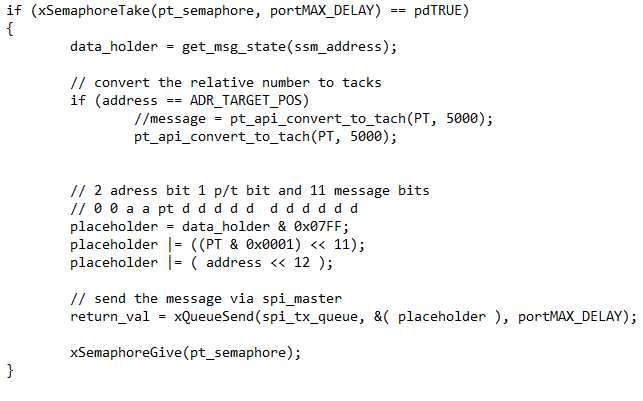
\includegraphics[scale=0.6]{Billeder/Micro_Controller/Semaphore_code_example.png}
\caption{ Semaphore code example }
\label{fig:Semaphore}
\end{figure}

First the process takes one semaphore. Then it takes another, do \textbf{SKRIV HVAD DEN GØR}. After that it releases the first semaphore and then the last. This insures that it has all the resources it needs to do its work and no deadlock is possible.











